\documentclass[a4paper,12pt]{article}

% --- Packages requis ---
\usepackage[utf8]{inputenc}
\usepackage[T1]{fontenc}
\usepackage[french]{babel}
\usepackage{graphicx}      
\usepackage{geometry}      
\usepackage{hyperref}      
\usepackage{float}         
\usepackage{parskip}       

\geometry{hmargin=2.5cm,vmargin=2.5cm}

\title{AI Models and Applications : Project Report\\
\large Celebrity Face Recognition Project}
\author{BEL HADJ Asmaa BEL HADJ \and VINCENT Valentin \and PHAM Kyllian}
\date{\today}

\begin{document}

\begin{titlepage}
    \centering
    
\includegraphics[width=0.5\textwidth]{logo-univ-cote-azur.png} % 
    \vspace{2cm}
    
    {\Large Master 1 Informatique\par}
    \vspace{1.5cm}
    
    {\Huge \textbf{AI Models and Applications : Project Report\\
\large Celebrity Face Recognition Project}\par}
    \vspace{2cm}
    
    {\Large \textbf{BEL HADJ Asmaa \\VINCENT Valentin\\PHAM Kyllian}\par}

    \vspace{0.5cm}
    {\Large \textbf{Superviseur :}\\ Enrico FORMENTI\par}
    
    \vfill
    {\large Université Côte d'Azur\par}
    {\large Année 2025-2026\par}
\end{titlepage}

\newpage
\tableofcontents
\newpage

%========================
\section{Introduction}
%========================

\subsection{Purpose of the Document}

This document aims to provide a detailed overview of the AI Models and Applications project. It outlines the challenges encountered, the solutions implemented, and the technical and the methodological choices that guided the development process.

\subsection{Project Overview}

This project, carried out as part of the AI Models and Applications course, focuses on recognizing celebrities in pictures based on their facial features. The project was coded in Python and by a group of three students: BEL HADJ BEL HADJ Asmaa, VINCENT Valentin and PHAM Kyllian.

The workflow is divided into three main steps. First, we use the yolo11n pre-trained network by Ultralytics to extract bounding boxes of people and store them in a dedicated “working” directory. Then, we employ the RetinaFace package to achieve pixel perfect bounding face extraction from these images. Finally, a pre-trained VGG network is used to identify the celebrities detected.

\subsection{Outline of the Report}

The structure of this report is organized as follows:

\begin{itemize}
    \item The first section provides an introduction, the project overview, and the purpose of this document.
    
    \item The second section introduces the first step of the project: extracting bounding boxes using yolo11n. It details the dataset, the chosen methodology and the associated technological choices.

    \item The third section focuses on the second step of the project: detecting and extracting faces using RetinaFace. It explains the processing of the extracted images and evaluates the accuracy of the detection.

    \item The fourth section describes the final stage of the project: implementing the pre-trained model network for celebrity recognition. It outlines the integration process and discusses the obtained results.

    \item The fifth section presents the Graphical User Interface (GUI) designed for the project.

    \item The sixth section presents the organization of the project.

    \item The final section, the conclusion, summarizes the key findings and opens the discussion to potential improvements.

    
\end{itemize}




\newpage

%========================
\section{Extracting Bounding Boxes}
%========================

The extraction of bounding boxes was realized using the Ultralytics library and the YOLO11n detection model. This model was chosen for its inference speed and simplicity of use.

YOLO (an acronym for You Only Look Once) is a real-time object detection system powered by deep learning. Unlike traditional methods that scan an image multiple times, YOLO processes the entire image in a single forward pass through the neural network. This allows it to simultaneously predict bounding boxes and class probabilities, making it exceptionally fast and efficient for high-speed applications without sacrificing significant accuracy.

The running pipeline is the following and is pretty straightforward :

\begin{enumerate}
    \item \textbf{Model initialization:} The process begins by loading the pre-trained YOLO11n model weights.

    \item \textbf{Inference execution:} A detection task is performed on an inputted image that contains one or multiple people.

    \item \textbf{Data parsing:} The model will return an array containing multiple elements and their information such as the element’s class number, coordinates, and more.

    \item \textbf{Class filtering:} We keep only the elements of class number 0, containing the information needed to segment each human detected in the image.

    \item \textbf{Region extraction and storage:} We extract all images using the coordinates and sizes provided in the array and save them into a directory named \texttt{img/working}.
\end{enumerate}

\begin{figure}[H]
\centering
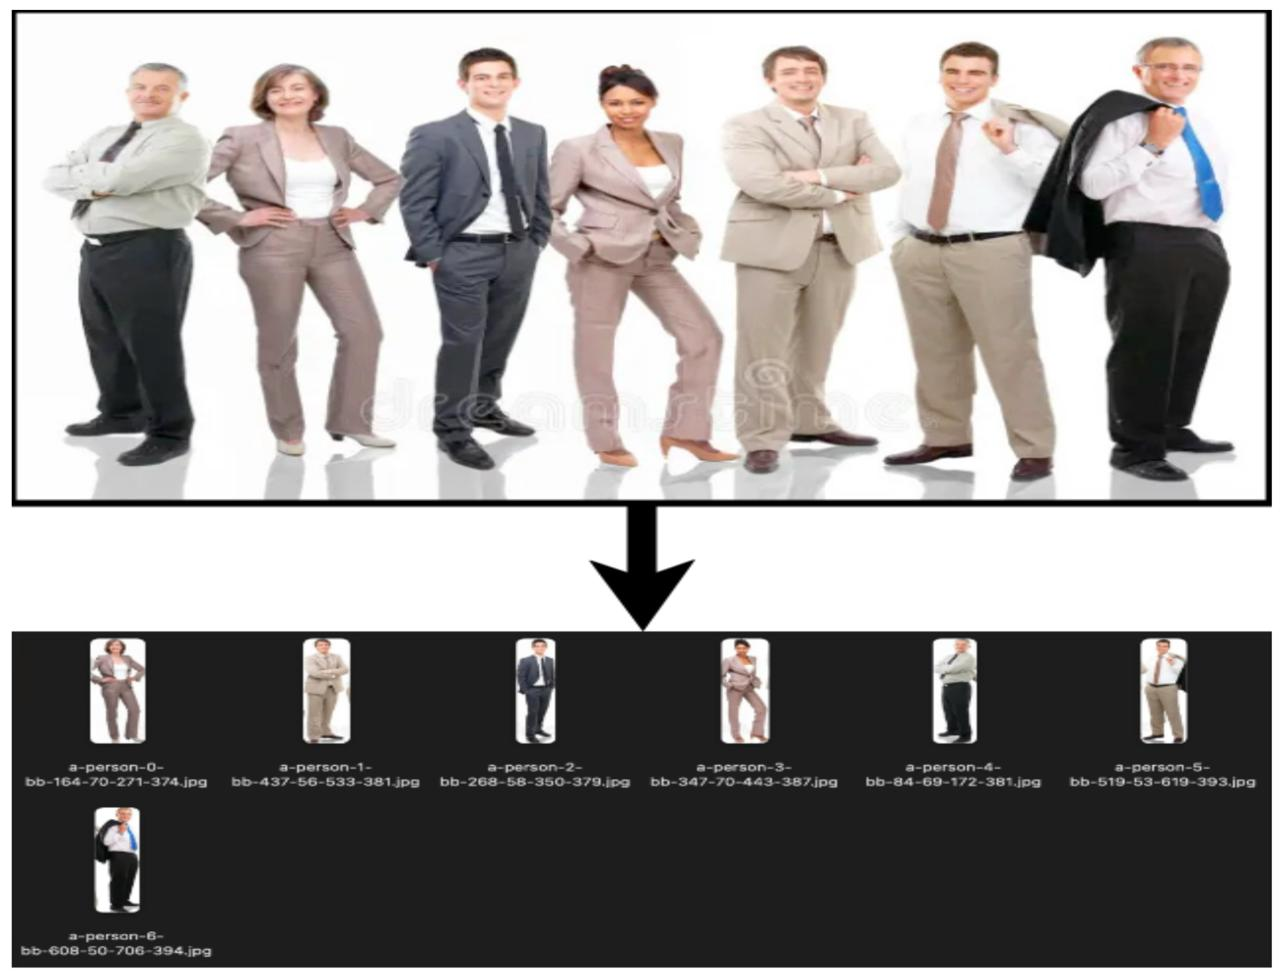
\includegraphics[width=0.7\textwidth]{WhatsApp Image 2026-01-22 at 20.30.39.jpeg}
\caption{Example of bounding box extraction using YOLO11n.}
\end{figure}

\newpage

%========================
\section{Faces Detection and Extraction using RetinaFace}
%========================

This section describes the implementation of the face detection and the extraction stage, which is handled in the Python script \texttt{extract\_faces.py}. The objective is to detect faces within the person crops generated by YOLO (situated in the \texttt{working} folder) and to extract clean, well-framed face images for the recognition stage.

The following libraries were used:
\begin{itemize}
    \item \textbf{RetinaFace :} face detection and landmark extraction.
    \item \textbf{PIL (Pillow) :} image loading and RGB conversion.
    \item \textbf{Numpy :} array manipulation and pixel-level processing.
    \item \textbf{os :} file and directory management.
    \item \textbf{json :} used for the serialization of the extracted metadata (age, emotion, …).
    \item \textbf{DeepFace :} analyses facial characteristics using a pre-trained model.
\end{itemize}



\subsection{Overview of RetinaFace Architecture}

As a requirement of this project, the RetinaFace model was used to detect and extract faces from the bounding boxes produced in the previous step. This  model based on deep learning  is widely recognized for its robustness and high accuracy. It detects faces with a high precision, delivers the position of the face as well as the facial landmarks (eye, nose,...) and a confidence score indicating detection reliability. RetinaFace analyzes an image at a pixel level, allowing it to locate faces accurately even if they are in a challenging position.

This method is essential for our project because it significantly reduces implementation complexity while ensuring high-quality detections. In my code, the function \texttt{detect\_faces()} from RetinaFace is used to obtain a dictionary containing all the details of the faces detected. 
This is an example of what it return for a single face detected:

\begin{figure}[H]
\centering
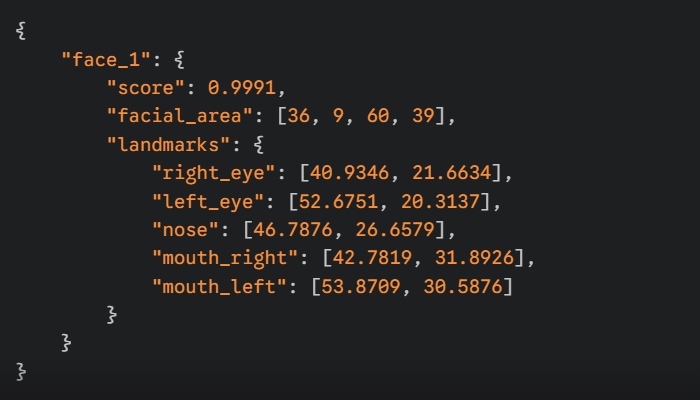
\includegraphics[width=0.7\textwidth]{dict_.png}
\caption{Example output from RetinaFace: face detection with confidence score, facial area, and landmarks.}
\end{figure}

\subsection{Dataset Preparation for Face Detection}

The images used at this stage come from the previous step, where yolo11n was used to detect persons and crop their bodies. These cropped images are stored in the “working” folder. 

Two main functions were implemented:
\begin{itemize}
    \item \textbf{\texttt{extract\_all\_faces\_in\_folder()}} : iterates through all person images and processes them one by one.
    \item \textbf{\texttt{extract\_faces()}} : detects and extracts faces from a single image.
\end{itemize}
The first function loops through the dataset and calls the second function for each image.

\subsection{Image Preprocessing and Cleaning}

Before extracting the faces, the raw detection output must be validated and cleaned. This step include: 
\begin{itemize}
    \item \textbf{\underline{Type verification:}} ensure that the output returned by RetinaFace is a dictionary.
    \item \textbf{\underline{Confidence filtering:}} keep only the detections with a confidence score superior or equal to 0.8 to ensure high-quality face results.
    \item \textbf{\underline{Boundary checking:}} use the functions \texttt{max()} and \texttt{min()} to reframe the faces situated in the image borders. This avoids errors of dimension occurring during the extraction stage.
    \item \textbf{\underline{Padding addition:}} add a padding of 15 pourcent around the detected face to improve lisibility and facilitate the cropping.
\end{itemize}
After these preprocessing steps, the faces are ready for extraction.

\subsection{Accuracy Evaluation and Error Analysis}

Although RetinaFace is highly robust, certain conditions can lead to hinder the analysis performed by DeepFace. The critical scenarios identified that may lead to failures in facial attribute extraction are the following:
\begin{itemize}
    \item \textbf{\underline{Low Resolution:}} if the extracted face is too small, the model may struggle to identify the features required for estimating age or emotion.
    \item \textbf{\underline{Extreme Poses:}} full profile faces often result in reduced accuracy or complete non-detection by \texttt{DeepFace}.
    \item \textbf{\underline{Motion Blur:}} this degrades the quality of the extracted attributes.
    \item \textbf{\underline{Overlapping:}} when multiple faces overlap or are partially covered by objects, facial landmarks become difficult to localize.
\end{itemize}
To ensure the resilience of the processing step, a robust error-handling strategy was implemented. A \texttt{try...except} block was integrated directly into the extraction loop of the \texttt{extract\_faces.py} script. This mechanism allows the program to catch exceptions raised by the method \texttt{DeepFace.analyse()} without interrupting the overall execution of the code. If the analysis fails for a specific face, the error is logged in the console, and the script automatically proceeds to the next image.

\subsection{Output Generation and Data structuring}

For extracting the faces, the Numpy array slicing is applied using the coordinates provided by RetinaFace. This approach isolates each detected face with precision.
To add an extra feature to the project, the DeepFace library is used to extract additional characteristics such as the age, dominant emotion and dominant gender. This is an example of what it return for a single face detected:

\begin{figure}[H]
\centering
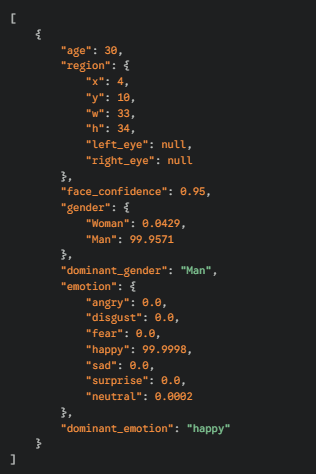
\includegraphics[width=0.7\textwidth]{facedeep.png}
\caption{Example output from DeepFace: facial attribute analysis.}
\end{figure}

The resulting data follow a rigorous hierarchical structure to ensure clarity and consistency.
\begin{itemize}
    \item Each result is centralized in the \texttt{faces} directory located at the root of the project.
    \item Each processed image has a dedicated subfolder automatically created.
    \item Inside this subfolder, the data are the following:
    \begin{itemize}
        \item an image containing the extracted face crop.
        \item a JSON file containing the corresponding extracted characteristics.
    \end{itemize}
\end{itemize}
This structure preserves a direct link between each face extracted and its metadata, thereby simplifying the next step of the project.

\newpage

\section{Celebrity Recognition}

This section describes how the face recognition script has been implemented using \texttt{Keras}, \texttt{TensorFlow} and the \texttt{VGG Face} library. The goal is to identify a celebrity based on their face (which has already been cropped) using a pre-trained model from Oxford University. This model was originally developed in \texttt{Caffe} or \texttt{Torch}, both of which are challenging to implement in \texttt{Python}. The library \texttt{keras\_vggface} is the \texttt{Python} implementation of the Oxford model, but it has not been maintained for a long time. It took significant effort to correctly configure an environment where this library could run (\texttt{Python}, \texttt{NumPy}, \texttt{OpenCV-Python} and \texttt{TensorFlow} had to be set to specific versions). All requirements can be found in \texttt{requirements.txt}, but here are the most important libraries being used:
\begin{itemize}
    \item \textbf{Keras :} High level API used to build and train neural network;
    \item\textbf{TensorFlow :} Google's open-source machine learning framework;
    \item\textbf{\texttt{keras\_applications} :} A module that provides pre-trained deep learning models like RESNET, VGG16, SESNET;
    \item \textbf{\texttt{keras\_vggface} :} library that provides pre-trained VGGFace model specifically designed for face recognition tasks;
    \item \textbf{Numpy :} array manipulation and pixel-level processing;
    \item \textbf{\texttt{opencv-python} :} tools for image and video processing, including reading/writing images.
\end{itemize}
To install the environment, \texttt{Anaconda} was used and an \texttt{INSTALL.md} file describes how to setup the environment. The script that triggers the face recognition is called \texttt{face\_recognition.py}. This \texttt{Python} script implements a celebrity face recognition system using a pre-trained \texttt{VGGFace} deep learning model (other models can also be tested, such as \texttt{RESNET50} and \texttt{SENET50}). The script processes a facial image and predicts which celebrity it most closely resembles from a database of known faces.

\subsection{Image Processing and Prediction}
The \texttt{predict\_celebrity()} function handles the entire prediction pipeline. It begins by loading an image from the specified file path using \texttt{OpenCV} and validates that the file exists. The image is then resized to $224 \times 224$ pixels, which is the required input dimension for \texttt{VGGFace} models. The image data is converted to a floating-point array and expanded to include a batch dimension, transforming it from a 3D tensor to a 4D tensor (image dimensions, number of colors, and batch size) as expected by the neural network.
Preprocessing is applied based on the selected model architecture. VGG16 uses version 1 preprocessing, while RESNET50 and SENET50 use version 2. This preprocessing step normalizes the pixel values according to the training procedure of each specific model, ensuring optimal performance. The preprocessed image is fed into the model to generate predictions, which are then decoded to retrieve the top celebrity matches.

\subsection{Models : VGG16, RESNET50, SENET50}

\begin{figure}[H]
\centering
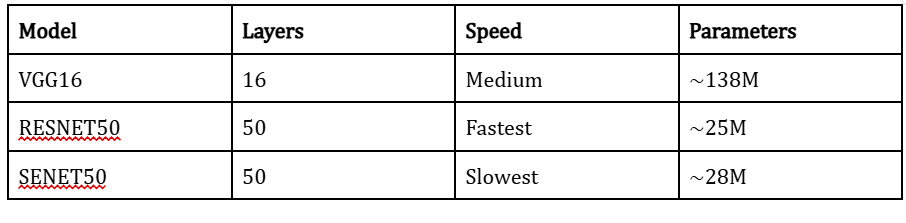
\includegraphics[width=1.0\textwidth]{tableau.png}
\caption{Comparison table of pre-trained models: VGG16, RESNET50, and SENET50.}
\end{figure}
A layer is step in face recognition analysis made by the neural network. It has only one job (for example analyses hair color, eye shape, etc). The more a model has layer the more accurate it should be. Parameters defines how score is calculated to match a celebrity face. For example : depending on hair darkness more point will be added to a celebrity score if the darkness matches. The number of parameters determines how the neural network memorize the faces it analyses. It can have a major impact since the number of parameters used determines the number of variations stored.

\subsection{Test case and conclusion}

In order to test our script, we used several pictures of celebrities. The three model were tested and only VGG face found the correct celebrity names. There is no cross references between both dataset (VGGFace used by VGG16 and VGGFace2 used by SENET50 and RESNET50). But in any case, only VGG16 did match the correct name for the pictures we tested. SENET50 and RESTNET50 failed constantly for pictures in their dataset.
This may be explained by the number of parameters used by VGG16 (138 millions). Storing more variation of each celebrity appearance can explain why it matched better than the others even if it is not expected.

\newpage

\section{GUI}

In order to have a way to implement the pipeline for people detection, facial segmentation and facial recognition, we decided to create a GUI to simplify the whole process for the user. 

To have a simple yet complete GUI, we decided to use the streamlit library that is a simple library to handle.

The GUI is pretty simple and straightforward, the user just needs to choose the model and upload an image and in the backend, we will do all the actions : 
\begin{enumerate}
    \item Extract the bodies in the image
    \item Extract the faces of every body detected
    \item Predict the celebrity detected
    \item Show the body, celebrity detected, the confidence of detection and some attributes (genre, age and emotion showed).
\end{enumerate}
Here is what the GUI is looking like,
When you start the script:
\begin{figure}[H]
\centering

\includegraphics[width=1.0\textwidth]{WhatsApp Image 2026-01-22 at 20.29.49.jpeg}
\caption{Overview of the Graphical User Interface (GUI) developed with Streamlit.}
\end{figure}

When you give a picture:
\begin{figure}[H]
\centering
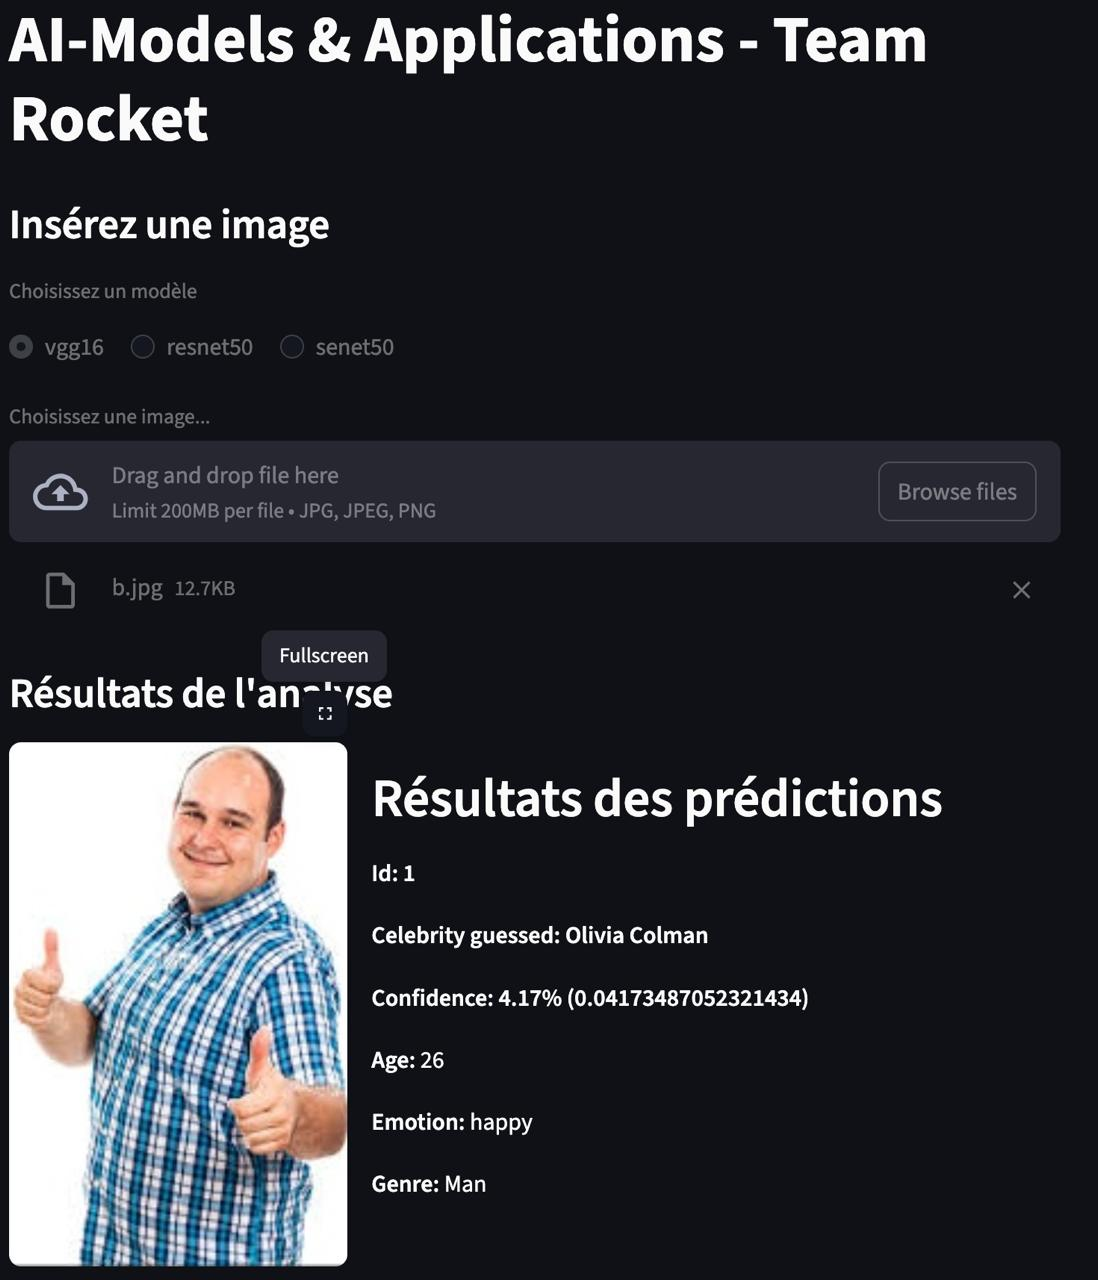
\includegraphics[width=1.0\textwidth]{WhatsApp Image 2026-01-22 at 20.30.07.jpeg}
\caption{Display of analysis results and celebrity predictions within the GUI.}
\end{figure}

\newpage
\section{Project Organization}
\subsection{Workflow Management}
To ensure smooth collaboration and rigorous code management, we relied on GitHub to organize our way of work. Our branching strategy was organized as follows:
\begin{itemize}
    \item \textbf{Individual branches:} each team member worked on a dedicated branch to develop their features independently, preventing interference with the work of others.
    \item \textbf{``dev'' branch:} this branch acted as an integration layer where we merged our respective contributions, tested modules and stabilized the application.
    \item \textbf{``main'' branch:} reserved for the final, stable and deliverable version of the project.
\end{itemize}
\subsection{Task Distribution}
The project was divided into three parts for each team member:
\begin{figure}[H]
\centering
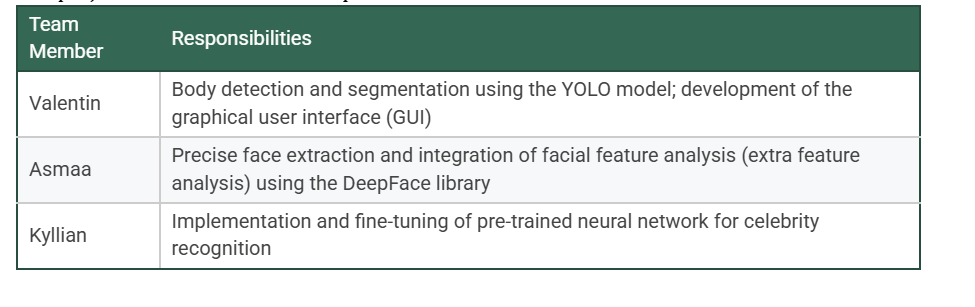
\includegraphics[width=1.1\textwidth]{tableau-2.png}
\caption{Distribution of tasks and responsibilities among team members.}
\end{figure}

\subsection{Code Management}
Respecting the project’s requirements, we organize our code in the following way:
\begin{itemize}
    \item \textbf{\texttt{persons/}} : This directory serves as the entry point, containing the untreated, raw images (.jpg) used for testing.
    \item\textbf{\texttt{pre/}} : This folder contains the preprocessing scripts, such as \texttt{bounding.py} for body extraction, \texttt{yolo11n.pt} (the YOLO model used by the bounding script to segment the bodies), and \texttt{extract\_faces.py} for facial extraction and attribute analysis.
    \item \textbf{\texttt{rep/}} : This directory is dedicated to the technical report and project documentation.
    \item \textbf{\texttt{src/}} : This folder contains the script for the Streamlit GUI \texttt{gui.py} and the celebrity recognition logic \texttt{face\_recognition.py}.
    \item \textbf{\texttt{img/working}} and \textbf{\texttt{faces/}} : These folders are dynamically generated during execution to store intermediate crops and final extracted face data with their respective JSON metadata.
    \item \textbf{\texttt{faces\_resnet\_50/}}, \textbf{\texttt{faces\_senet\_50/}}, and \textbf{\texttt{faces\_vgg\_16/}} : These folders contain images that work and don't work for each model.
\end{itemize}

\newpage

\section{Conclusion}
\subsection{Project Summary}
This project successfully designed and implemented a complete processing pipeline for celebrity recognition. By integrating YOLO11n for person detection, RetinaFace for high-precision face extraction and VGGFace for identity prediction, we transformed raw images into structured and analyzable data. Furthermore, the integration of attribute analysis and a graphical interface added a layer of depth to the project.

\subsection{Problems encountered}
The development of this project was marked by two major technical challenges: 
\begin{itemize}
    \item \textbf{\underline{Dependency Management:}} managing dependencies proved particularly complex. Using older libraries alongside modern versions of \texttt{TensorFlow} and \texttt{NumPy} required the creation of isolated environments to ensure a stable system.
    \item \textbf{\underline{Input data quality:}} recognition accuracy highly depended on the quality of the input images. Although \texttt{RetinaFace} is robust for detection, the recognition model remains sensitive to extreme poses and low resolution, which often lead to reduced confidence scores.
    \item \textbf{\underline{Poor result:}} We had much more difficulty finding examples where the \texttt{RESNET50} and \texttt{SENET50} models give the correct result than with the \texttt{VGG16} model. The larger volume of data in the \texttt{VGGface2} dataset used by \texttt{RESNET50} and \texttt{SENET50} may be the cause.
\end{itemize}

\subsection{Areas for Improvement}
To further improve this project, several features could be considered:
\begin{itemize}
    \item \textbf{\underline{Real-time Optimization:}} The current pipeline processes static images. Adding support for video stream processing would be an interesting way to elevate the project.
    \item \textbf{\underline{Fine-tuning:}} Retraining the final layers of \texttt{RESNET50} on a more contemporary celebrity dataset could improve its accuracy and potentially yield better results.
    \item \textbf{\underline{Advanced GUI:}} Improving the current graphical interface by adding real-time comparative analytics between different models would provide a more informative and interactive user experience.
\end{itemize}

\end{document}
